%\documentclass[spanish]{beamer}

\documentclass{beamer}
\usepackage{pgf,pgfpages}
%\pgfpagesuselayout{4 on 1}[letterpaper,landscape,border shrink=0.5in]
\usepackage{algorithm,algorithmic}
%\usepackage{algorithm,algorithmicx}
%\usepackage[noend]{algpseudocode}
\usepackage{listings}
\lstset{basicstyle=\ttfamily,
	showstringspaces=false,
	commentstyle=\color{red},
	literate={á}{{\'a}}1
	{ã}{{\~a}}1
	{é}{{\'e}}1
	{ó}{{\'o}}1
	{í}{{\'i}}1
	{ñ}{{\~n}}1
	{¡}{{!`}}1
	{¿}{{?`}}1
	{ú}{{\'u}}1
	{Í}{{\'I}}1
	{Ó}{{\'O}}1
}

\usepackage{beamerthemesplit}
\usepackage{color}
\usepackage[utf8]{inputenc}
\usepackage[spanish]{babel}
%\usepackage[latin1]{inputenc}
%\usepackage[pdftex]{graphicx}
%\usepackage{algorithm}
%\usepackage{algorithmic-C}
%\usepackage{algorithmic}
\usepackage{amsthm}
\usepackage{multicol}
\usepackage{multirow}
\usepackage{fancyvrb,relsize}
\usepackage{hhline}
\usepackage{tikz}
\usetikzlibrary{trees, shapes, calc}
\newcommand{\inputTikZ}[2]{%
	\scalebox{#1}{\input{#2}}
}

\usetheme{Warsaw} %Gueno
%\usetheme{Darmstadt} %OK!
% \usetheme{Frankfurt} %OK!
%\usetheme{Goettingen}
%\usetheme{Dresden}
%\usetheme{JuanLesPins} %OK!!
%\usetheme{Marburg}
%\usetheme{Montpellier}
%\usetheme{Rochester} %sobrio
%\usetheme{Singapore}
%\usetheme{Szeged}

%\usecolortheme{albatross}
%\usecolortheme{seahorse}
%\usecolortheme{beetle}
%\usecolortheme{crane}
%\usecolortheme{dolphin}
%\usecolortheme{dove}
%\usecolortheme{fly}
%\usecolortheme{lily} %Gueno
\usecolortheme{orchid}%Gueno
%\usecolortheme{rose}
%\usecolortheme{seagull}
%\usecolortheme{whale}


\DefineVerbatimEnvironment%
      {VerbatimNN}%
      {Verbatim}%
      {fontsize=\relsize{-1}}
\DefineVerbatimEnvironment%
      {VerbatimNNN}%
      {Verbatim}%
      {fontsize=\relsize{-2}}

\DefineVerbatimEnvironment%
      {VerbatimPseudo}%
      {Verbatim}%
      {numbers=left, fontsize=\relsize{-1}}
\DefineVerbatimEnvironment%
      {VerbatimPseudoReduced}%
      {Verbatim}%
      {numbers=left, fontsize=\relsize{-2}}
\DefineVerbatimEnvironment%
      {VerbatimPseudoReduced2}%
      {Verbatim}%
      {numbers=left, fontsize=\relsize{-3}}
\DefineVerbatimEnvironment%
      {VerbatimC}%
      {Verbatim}%
      {commandchars=@ªº, numbers=left, fontsize=\relsize{-1}}
\DefineVerbatimEnvironment%
      {VerbatimReducedC}%
      {Verbatim}%
      {commandchars=@ªº, numbers=left, fontsize=\relsize{-2}}
\DefineVerbatimEnvironment%
      {VerbatimReduced2C}%
      {Verbatim}%
      {commandchars=@ªº, numbers=left, fontsize=\relsize{-3}}



%\AtBeginSubsection[]
%{
% \begin{frame}
% \frametitle{Sinopsis}
% Aqui decides: cada seccion y subseccion:
% \tableofcontents[currentsection,currentsubsection]
 %O solamente la seccion (Solo uno de ellos)
%\tableofcontents[currentsection]
% \end{frame}
%}

% Si quieres que todo por default aparezca de poco en poco
% descomenta esta linea
%\beamerdefaultoverlayspecification{<+->}

\setbeamertemplate{footline}{\hfill\insertframenumber/\inserttotalframenumber}
\setbeamertemplate{navigation symbols}{}

\setbeamercovered{transparent}

\title{ELO320 - Estructuras de Datos y Algoritmos\\Introducción a C\\Expresiones y Estructuras de Control}
%\subtitle{Ingeniería Civil Telemática UTFSM}
\author{Dr. Nicolás Gálvez R.\\{\small nicolas.galvez@usm.cl}}
\institute{Ing. Civil Telemática - Departamento de Electrónica}
\titlegraphic{
\includegraphics[scale=.145]{images/logoutfsm}}
\date{1er Semestre 2025}

\begin{document}

\frame{\titlepage}

%\section*{Sinopsis}
%\frame{  \frametitle{Sinopsis}\tableofcontents[pausesections]}
%
%

%\section{¿Por qué C?}
%
%\begin{frame}{Programación Estructurada}
%	\begin{block}{}
%		{\small\textbf{Paradigma de programación} basado en el \textbf{uso extensivo de subrutinas y estructuras de control}, con el fin de mejorar la \textbf{claridad}, \textbf{calidad} y \textbf{tiempo de desarrollo} del código de programas computacionales.}
%	\end{block}
%	\begin{itemize}
%		\item \textbf{C, lanzado en 1973, es el mayor exponente de este tipo de lenguajes.}
%	\end{itemize}
%	\vspace{-.25cm}
%	\begin{center}
%		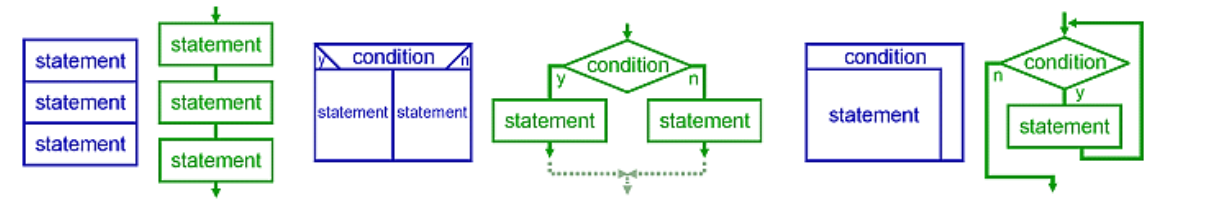
\includegraphics[width=\linewidth]{images/structured.png}
%	\end{center}
%\end{frame}
%
%\begin{frame}{¿Por qué es C tan relevante?}
%\begin{itemize}
%\item Diseñado para desarrollar UNIX OS
%\item Maneja actividades de bajo nivel (en la memoria), a pesar de ser un lenguaje de alto nivel.
%\item Se relaciona eficientemente con instrucciones de máquina.
%\item Perdura su uso en el tiempo.
%\item La mayoria de software tiene una relación directa o indirecta con C.
%\end{itemize} 
%\end{frame}
%
%\section{Elementos Generales}
%\begin{frame}[fragile]{Elementos Generales - Datos}
%\begin{itemize}
%	\footnotesize
%	\item \textbf{Datos Primitivos:} enteros, reales, caracteres.
%	\vspace{-.45cm}
%	\begin{columns}[t]
%		\begin{column}{5.1cm}
%		\begin{exampleblock}{C}
%		\begin{lstlisting}[language=C,basicstyle=\scriptsize]
%int contador = 10;
%char nombre[10] = "Eduardo";
%float PI = 3.14159;
%		\end{lstlisting}
%		\end{exampleblock}
%		\end{column}
%		\begin{column}{5.1cm}
%		\begin{block}{Python}
%		\begin{lstlisting}[language=Python, basicstyle=\scriptsize]
%contador = 10
%nombre = "Eduardo"
%PI = 3.14159
%		\end{lstlisting}
%		\end{block}
%		\end{column}
%	\end{columns}
%	\vspace{.15cm}
%	\item \textbf{Estructurados:} agrupar/componer conjuntos de datos del mismo tipo en una unidad (e.g. Arreglo). 
%	\vspace{-.45cm}
%	\begin{columns}[t]
%		\begin{column}{5.1cm}
%		\begin{exampleblock}{C}
%		\begin{lstlisting}[language=C,basicstyle=\scriptsize, escapeinside={|}{|}]
%char semana[5][20] =
%{"Lu","Ma","Mi","Ju","Vi"};
%printf("|\%s|\n", semana[1]);
%		\end{lstlisting}
%		\end{exampleblock}
%		\end{column}
%		\begin{column}{5.1cm}
%		\begin{block}{Python}
%		\begin{lstlisting}[language=Python,basicstyle=\scriptsize]
%semana = ["Lu","Ma","Mi",
%          "Ju","Vi"]
%print(semana[1])
%		\end{lstlisting}
%		\end{block}
%		\end{column}
%	\end{columns}
%	\vspace{.15cm}
%\end{itemize}
%\end{frame}
%
%\begin{frame}[fragile]{Elementos Generales - Estructuras de Control}
%\small
%\vspace{-.25cm}
%	\begin{itemize}
%		\footnotesize
%		\item \textbf{Sentencias:} abstrae conjunto de instrucciones.
%		\item \textbf{Estructuras de control:} secuenciación, condición y repetición (e.g. if, while).
%		\item \textbf{Abstracción procedural:} procedimiento con un nombre y parámetros (e.g. funciones y métodos).
%		\item \textbf{Concurrencia:} computación paralela (e.g. procesos y hebras). 
%	\end{itemize}
%	\small
%\end{frame}
%
%\begin{frame}[fragile]{Métodos de Implantación}
%\begin{itemize}
%	\item \textbf{Com%pilación:} (e.g. C, C++)\\
%	Traduce a lenguaje de máquina para posterior ejecución (interpretación directa por el procesador).
%	\item \textbf{Interpretación:} (e.g. LISP, Python)\\
%	Una máquina virtual interpreta directamente el código fuente durante la ejecución.
%	\item \textbf{Híbrido:} (e.g. Java, C\#)\\
%	Se compila a un lenguaje intermedio, que luego es interpretado.
%\end{itemize}
%\end{frame}
%
%\begin{frame}[fragile]{Uso de Código en C}
%\large
%\begin{itemize}
%	\item \textbf{Modularización:} descomponer programas en unidades de desarrollo más pequeñas (módulos). 
%	\item \textbf{Compilación Separada o Indepediente:} Módulos de un programa se pueden compilar por separado (bibliotecas).
%	\item \textbf{Reutilización:} Módulos y clases se pueden reutilizar para diferentes programas. 
%\end{itemize}
%\end{frame}
%
%\begin{frame}[fragile]{Popularidad de Lenguajes (stackoverflow, redmonk)}
%\vspace{-.25cm}
%\begin{center}
%	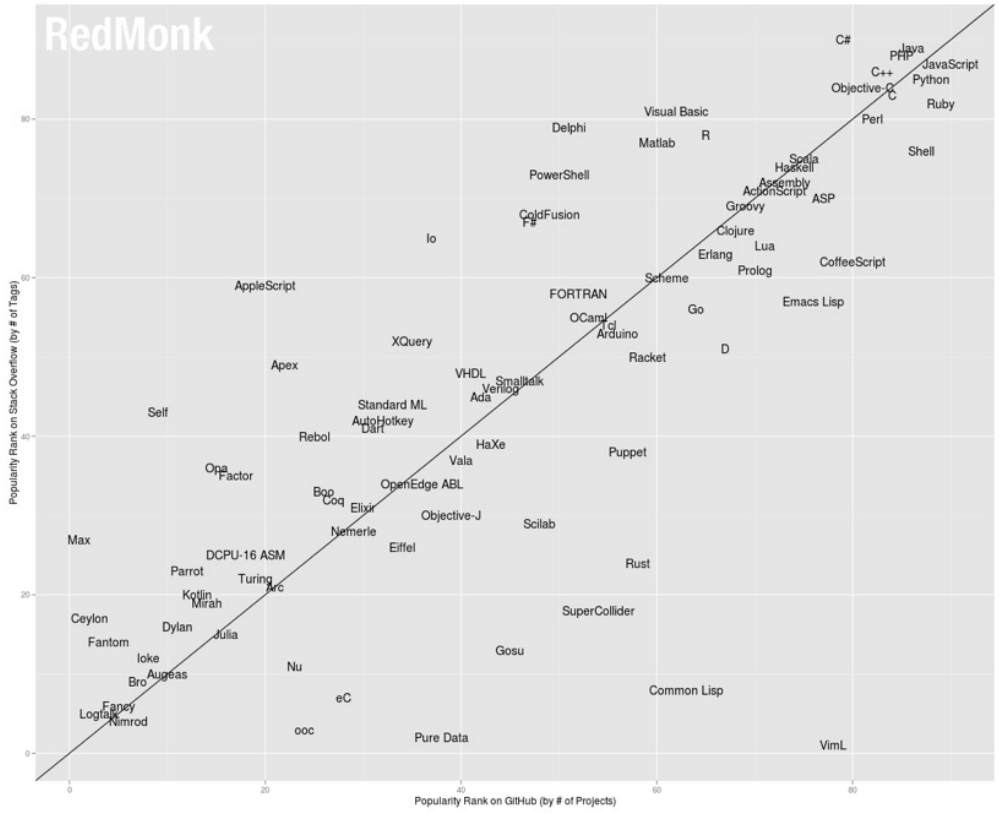
\includegraphics[width=.9\linewidth]{images/01-popularity.png}
%\end{center}
%\end{frame}
%
%\begin{frame}[fragile]{Rendimiento de Lenguajes}
%\begin{center}
%	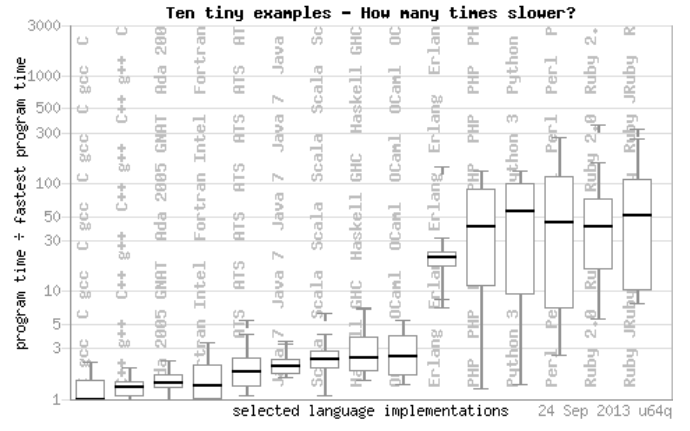
\includegraphics[width=.7\linewidth]{images/01-benchmark.png}
%\end{center}
%
%%\Large
%\url{http://benchmarksgame.alioth.debian.org/u32/performance.php}
%\end{frame}

%\section{Aprendamos C}
%\part{Base}
%\subsection{Estructura General}
%\begin{frame}[fragile]{C Estructura general}
%\begin{itemize}
%	\item Requiere un método de inicio de ejecución: \textbf{main}
%\end{itemize}
%
%%\vspace{-.45cm}
%%  \begin{columns}[t]
%%\begin{column}{5.1cm}
%\begin{exampleblock}{C}
%\begin{lstlisting}[language=C,basicstyle=\scriptsize]
%#include<stdio.h>
%
%int main() {
%	printf("Hola Mundo\n");
%	return 0;
%}
%\end{lstlisting}
%\end{exampleblock}
%%\end{column}
%%\begin{column}{5.1cm}
%\begin{block}{Python}
%	\begin{lstlisting}[language=Python,basicstyle=\scriptsize]
%if __name__ == "__main__":
%	print("Hola Mundo!")
%	\end{lstlisting}
%\end{block}
%%\end{column}
%%\end{columns}
%\end{frame}
%
%\begin{frame}[fragile]{Compilación: gcc}
%C es un lenguaje compilado, esto significa que: 
%\begin{itemize}
%\item Su código es transformado, a través de un compilador, a lenguaje máquina.
%\item El resultado de la compilación es un binario ejecutable. 
%\item Binarios ejecutables: .bin, .exe, .appinstall, etc.
%\end{itemize}
%
%\begin{figure}[h!]
%\begin{center}
%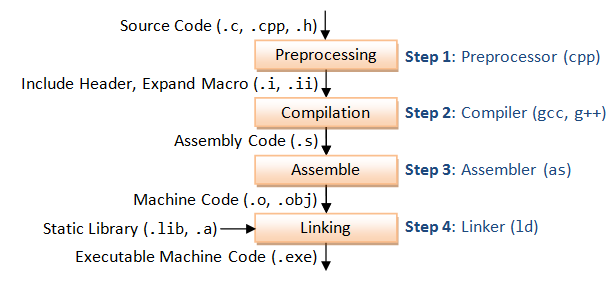
\includegraphics[width=0.7\textwidth]{images/gcc}
%\end{center}
%\end{figure}
%
%\end{frame}
%
%\begin{frame}[fragile]{Compilación: gcc}
%
%Quizas la imagen anterior ahora tenga mayor sentido: 
%\bigskip
%\begin{figure}[h!]
%\begin{center}
%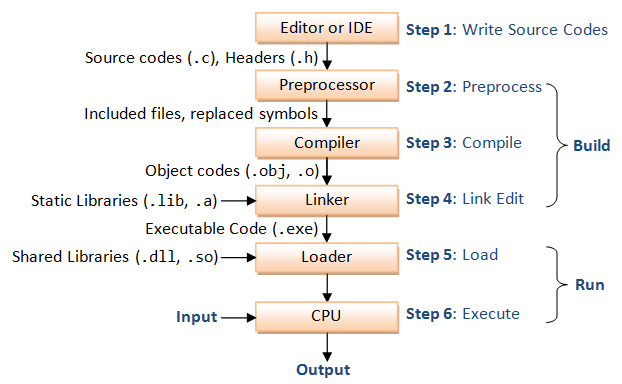
\includegraphics[width=0.7\textwidth]{images/gcc-win}
%\end{center}
%\end{figure}
%\end{frame}
%
%\begin{frame}[fragile]{Compilación: gcc}
%
%\begin{alertblock}{Compliación directa}
%\begin{lstlisting}[language=bash, basicstyle=\scriptsize, escapeinside={|}{|}]
%[user@pc dir]|\$| gcc -o ejecutable codigo1.c codigo2.c -Wall
%\end{lstlisting}
%\end{alertblock}
%{\footnotesize
%donde:
%\begin{itemize}
%\item \textbf{-o} (output) indica que lo siguiente es el nombre del ejecutable.
%\item \textbf{codigoX.c} es el archivo de nuestro código (pueden ser más de uno)
%\item \textbf{-Wall} indica que el compilador de aviso de potenciales peligros (warnings)
%\end{itemize}
%}
%\end{frame}
%
%\begin{frame}[fragile]{Compilación: gcc}
%
%\begin{exampleblock}{Compilación por pasos}
%\begin{lstlisting}[language=bash, basicstyle=\scriptsize, escapeinside={|}{|}]
%[user@pc dir]|\$| gcc -c codigo1.c -Wall
%[user@pc dir]|\$| gcc -c codigo2.c -Wall
%[user@pc dir]|\$| gcc -o ejecutable codigo1.o codigo2.o 
%\end{lstlisting}
%\end{exampleblock}
%{\footnotesize
%donde:
%\begin{itemize}
%\item \textbf{-c} indica que un archivo.c será compilado independientemente a un archivo objeto .o.
%\item \textbf{-o} (output) indica que lo siguiente es el nombre del ejecutable. 
%\item \textbf{-Wall} indica que el compilador de aviso de potenciales peligros (warnings)
%\item En la última instrucción se enlazan todos los archivos compilados de forma independiente. 
%\end{itemize}
%}
%\end{frame}
%
%
%\subsection{Tipos de datos}
%\begin{frame}[fragile]{Tipificación de Datos - Explícita VS Implícita}
%\begin{itemize}
%	\item Exigencia en la declaración para detectar potenciales errores de tipo.
%	\item \textbf{Tipificación explícita (C): } 
%	\begin{itemize}
%		\item Siempre detecta errores de tipo. 
%		\item Restricciones sobre operaciones y valores de diferentes tipos de datos.
%		\item No hay ejecución si tipos son erróneos. 
%		\item Tipificación estática y explícita.
%	\end{itemize}
%	\item \textbf{Tipificación implícita (Python): } 
%	\begin{itemize}
%		\item Conversiones que permiten relajar restricciones.
%		\item Flexibilidad y agilidad.
%		\item Genera errores no detectados.
%	\end{itemize}
%	
%\end{itemize}
%\end{frame}
%
%\begin{frame}[fragile]{Tipos de datos en C}
%\begin{itemize}
%	\item Se define qué tipo de dato es cada variable antes de usarlas (tipificación explícita):
%	\begin{exampleblock}{C}
%		\begin{lstlisting}[language=C,basicstyle=\scriptsize,escapeinside={|}{|}]
%#include<stdio.h>
%
%int main() {
%	int a;
%	float d;
%	int b = 5, c = 6;
%	printf("|\%|d\n", b+c);
%	return 0;
%}
%		\end{lstlisting}
%	\end{exampleblock}
%	\item En Python los tipos de datos se infieren de la asignación (tipificación implícita).
%\end{itemize}
%\end{frame}
%
%\begin{frame}[fragile]{Tipos de datos primitivos en C}
%\vspace{-.25cm}
%\begin{center}
%	%  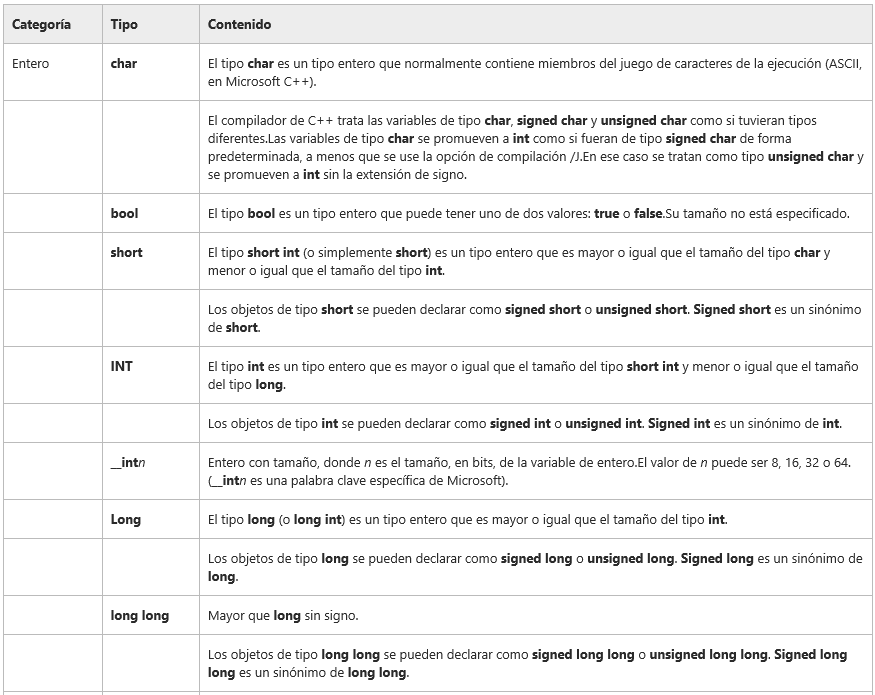
\includegraphics[width=.94\linewidth]{images/VarTypes_1.PNG}
%	\begin{tabular}{|l|l|l|}\hline \hline
%		\textbf{Descripción} & \textbf{C} & \textbf{Python}   \\ \hline \hline
%		Booleano       &  bool &  bool \\
%		Byte           &  char  & int \\
%		Caracter       &  char  & str \\
%		Entero corto   &  short & int \\
%		Entero         &  int  & int \\
%		Entero largo   & long  & long \\
%		Punto flotante & float & float   \\
%		Pto. flotante largo & double & float   \\
%		String              & - & str \\ 
%		Complejos  & - & complex \\ \hline
%	\end{tabular}
%\end{center}
%\end{frame}
%
%\begin{frame}[fragile]{Tipos de datos primitivos en C}
%\vspace{-.25cm}
%\begin{center}
%	%  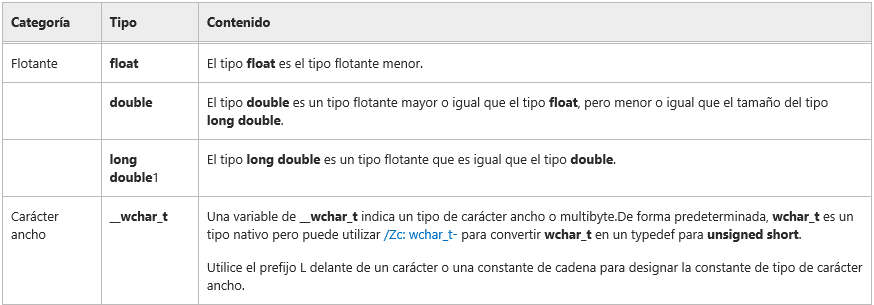
\includegraphics[width=.94\linewidth]{images/VarTypes_2.PNG}
%	\small
%	\begin{tabular}{|l|l|l|}\hline \hline
%		tipo & bytes & Rango\\ \hline 
%		char & 1 & -127 to 127 or 0 to 255\\ \hline 
%		unsigned char & 1 & 0 to 255\\ \hline 
%		signed char & 1 & -127 to 127\\ \hline 
%		int & 4 & -2147483648 to 2147483647\\ \hline 
%		unsigned int & 4 & 0 to 4294967295\\ \hline 
%		signed int & 4 & -2147483648 to 2147483647\\ \hline 
%		short int & 2 & -32768 to 32767\\ \hline 
%		unsigned short int & 2 & 0 to 65,535\\ \hline 
%		signed short int & 2 & -32768 to 32767\\ \hline 
%		long int & 4 & -2,147,483,647 to 2,147,483,647\\ \hline 
%		signed long int & 4 & same as long int\\ \hline 
%		unsigned long int & 4 & 0 to 4,294,967,295\\ \hline 
%		float & 4 & +/- 3.4e +/- 38 (~7 digits)\\ \hline 
%		double & 8  & +/- 1.7e +/- 308 (~15 digits)\\ \hline 
%		long double & 8  & +/- 1.7e +/- 308 (~15 digits)\\ \hline 
%	\end{tabular}
%\end{center}
%\end{frame}
%
%\begin{frame}[fragile]{Tipos de Datos}
%\begin{itemize}
%	\item \textbf{Sistema de tipificación en C:}
%	\begin{itemize}
%		\item \textbf{Verificación de tipo:} Los operandos de una operacion deben ser de \emph{tipo compatible}.
%		\item \textbf{Tipo compatible:} es un tipo permitido, o que puede ser convertido en uno permitido.
%		\item \textbf{Conversión de tipos:} \emph{Coerción} es conversión automática y \emph{casting} es la conversión definida por el programador.
%		\begin{lstlisting}[language=C]
%int pi = 3.14;          //coerción
%double d = (double) pi; //casting       
%		\end{lstlisting}
%		\item \textbf{Error de tipo:} aplicación de un tipo inapropiado en una instrucción.
%	\end{itemize}
%\end{itemize}
%\end{frame}
%\part{I/O}
%\subsection{Entradas y Salidas}
%
%\begin{frame}{Especificadores}
%Las funciónes de I/O de C utilizan especificadores para identificar el tipo de dato a leer o imprimir:
%
%\begin{center}
%	\small
%	\begin{tabular}{|l|l|}\hline \hline
%	Tipo & Especificador\\ \hline
%	char & \%c \\\hline
%	int & \%d \hspace{0.3cm} \%i \\\hline
%	unsigned int & \%u \\\hline 
%	float & \%f \hspace{0.2cm} \%.3f \\\hline
%	string & \%s \\\hline
%	double & \%lf \\\hline
%	long int & \%ld \\\hline
%	long long unsigned int & \%Lu \\\hline
%	\end{tabular}
%\end{center}
%\end{frame}
%
%\begin{frame}[fragile]{Entrada Estándar: scanf}
%Función de entrada estándar,  se compone de una sección de especificadores y otra sección de variables a asignar el valor leído.
%
%\begin{exampleblock}{scanf}
%\begin{lstlisting}[language=C,basicstyle=\scriptsize,escapeinside={|}{|}]
%int a;
%char c;
%char nom[10];
%double prec;
%
%scanf("|\%|d", |\&|a); //lee un entero
%scanf("|\%|c", |\&|c); //lee un char
%scanf("|\%|s", nom); //lee un string
%
%//lee un double, un string y un entero.
%scanf("|\%|lf |\%|s |\%|d", |\&|prec, nom, |\&|a); 
%\end{lstlisting}
%\end{exampleblock}
%\end{frame}
%
%\begin{frame}[fragile]{Salida Estándar: printf}
%Función de salida estándar, se compone de una sección de especificadores y otra sección de variables cuyos valores se mostrarán.
%
%\begin{exampleblock}{printf}
%\begin{lstlisting}[language=C,basicstyle=\scriptsize,escapeinside={|}{|}]
%printf("|\%|d", a); //imprime un int
%printf("|\%|c", c); //imprime un char
%printf("|\%|s", nom); //imprime un string
%
%//imprime un double de 3 decimales, un string y un entero.
%printf("|\%|.3lf |\%|s |\%|d", prec, nom, a); 
%\end{lstlisting}
%\end{exampleblock}
%
%\end{frame}
%
%
%\subsection{Asignaciones e Inicialización}
%\begin{frame}[fragile]{Definir $\neq$ Asignar $\neq$ Inicializar}
%\begin{exampleblock}{C}
%	\begin{lstlisting}[language=C,basicstyle=\scriptsize,escapeinside={|}{|}]
%#include<stdio.h>
%int main(){
%	int a; //Define a la variable a como tipo entero
%	a = 3 + 2; //Evalúa 3+2 que es 5 y se asigna a 'a'. 
%	printf("|\%|d\n", a);
%	return 0;
%}
%	\end{lstlisting}
%\end{exampleblock}
%\end{frame}
%\begin{frame}[fragile]{Definir $\neq$ Asignar $\neq$ Inicializar}
%%\vspace{-.25cm}
%%\large 
%\small En C soporta el uso de ambos conceptos (definición y asignación) en conjunto. A esto se llama inicialización.
%\begin{exampleblock}{C}
%	\begin{lstlisting}[language=C,basicstyle=\scriptsize,escapeinside={|}{|}]
%#include<stdio.h>
%int main(){
%	int a = 3 + 2; 
%	printf("|\%|d\n", a); // Inicializa con resultado 3+2
%	return 0;
%}
%	\end{lstlisting}
%\end{exampleblock}
%
%\end{frame}
%
%\begin{frame}[fragile]{Enumeración}
%\small
%	\begin{exampleblock}{C} 
%	\begin{lstlisting}[language=C,basicstyle=\scriptsize,escapeinside={|}{|}]
%enum color {
%	rojo, 
%	amarillo, 
%	verde=20, 
%	azul};
%
%int col = rojo;
%
%if (col != azul){ 
%	printf("No es azul\n");}
%	\end{lstlisting}\end{exampleblock}
% \begin{block}{Python (clases)}
%	\begin{lstlisting}[language=Python,basicstyle=\scriptsize]
%class Colors(Enum):
%	red = 1
%	yellow = 2
%	green = 3
%	\end{lstlisting}\end{block}
%\end{frame}
%
%\subsection{Preview Próx. Clases}
%\begin{frame}[fragile]{Preview Próx. Clases: Arreglos y Strings}
%\small
%\begin{itemize}
%	\item \textbf{Arreglo:} Tipo estructurado consistente en conjunto homogéneo y ordenado de elementos.
%	\item Se identifican por su posición relativa mediante un \emph{índice} encerrado con paréntesis cuadrados (parte de índice 0).
%	\begin{lstlisting}[language=C,basicstyle=\scriptsize,escapeinside={|}{|}]
%//Arreglos estáticos (se liberan al terminar 
%// el ámbito donde fueron declaradas):
%int foo[10]; //10 enteros creados en foo.
%foo[3] = 7; //A cuarto elemento se asigna un 7.
%	\end{lstlisting}
%	
%	\item \textbf{String:} Arreglo de caracteres.
%	\begin{lstlisting}[language=C,basicstyle=\scriptsize,escapeinside={|}{|}]
%// Los string se delimitan con caracter '\0' 
%// (requiere espacio de 1 char):
%char nombre[10] = "Juan"; //String de largo máximo 10. 
%nombre[1] = 'e'; //Qué hace? 
%printf("|\%|s\n", nombre);
%	\end{lstlisting}
%
%	\item Veremos más sobre arreglos la próxima clase. 	
%\end{itemize}
%\end{frame}

%\begin{frame}[fragile]{Operaciones sobre Strings}
%Para operaciones sobre arreglos de caracteres, se debe incluir la biblioteca \textbf{cstring}.\\
%
%\begin{itemize}
%\item \textbf{C/C++}
%\end{itemize}
%\begin{lstlisting}[language=C++]
%
%#include <cstring>
%//...
%char str1[10] = "hola ";
%char str2[10] = "mundo";
%// Imprime 5
%std::cout<<strlen(str1)<<std::endl; 
%// Imprime "hola mundo"
%std::cout<<strcat(str1,str2)<<std::endl; 
%strcpy(str1,str2);
%// Imprime "mundo"
%std::cout<<str1<<std::endl; 
%\end{lstlisting}
%\end{frame}
%
%\begin{frame}[fragile]{Operaciones sobre Strings}
%\begin{itemize}
%\item \textbf{Equivalentes en Python}
%\begin{lstlisting}[language=Python]
%#...
%str1 = "hola "
%str2 =  "mundo"
%# Imprime 5
%print(len(str1))
%# Imprime "hola mundo"
%print(str1 + str2)
%str1 = str2
%# Imprime "mundo"
%print(str1)
%#...
%\end{lstlisting}
%\end{itemize}
%\end{frame}
%
%\begin{frame}[fragile]{Tipos de Datos Abstractos - Estructuras}
%\begin{itemize}
%	\item Conjunto (posiblemente) heterogéneo de elementos de datos (e.g.: estructuras y clases).
%	\item Cada elemento individual (campo, miembro o atributo) identificado con un nombre. 
%	\item Encapsulamiento de información.
%	\item Ejemplo:
%	\begin{lstlisting}[language=C++]
%struct empleado {
%    char nombre[40];
%    char ap_paterno[40];
%    char ap_materno[40];
%    float sueldo;
%};
%//...
%empleado e1, e2;
%
%//Acceso a atributos con operador '.'
%e1.sueldo = 550000.00;
%strcpy(e1.nombre, "Juan");
%	\end{lstlisting}
%\end{itemize}
%\end{frame}
\part{Clase Activa}
\section{Clase Activa}
\begin{frame}[fragile]{Clase Activa: Módulo 1}
\begin{exampleblock}{Ejercicio 1.1}
Cree un programa que solicite por pantalla una temperatura en grados Fahrenheit y arroje como resultado su transformación a Grados Celsius.

$$ {^\circ}C = \frac{5}{9} \times ({^\circ}F - 32) $$
\end{exampleblock}

{\tiny Aprendemos: Entrada y Salida, Tipos de Datos, Conversiones, Operadores Aritméticos.}
\end{frame}

\begin{frame}[fragile]{Clase Activa: Módulo 1}
\begin{exampleblock}{Ejercicio 1.2}
Cree un programa que solicite por pantalla una temperatura en grados Celsius y pregunte si quiere como resultado su transformación a Grados Fahrenheit o Kelvin.

$$ {^\circ}K = {^\circ}C + 273.15 $$
\end{exampleblock}

{\tiny Aprendemos: control condicional, if, u opciones, switch.}
\end{frame}

\begin{frame}[fragile]{Clase Activa: Módulo 1}
\begin{exampleblock}{Ejercicio 1.3}
Cree un programa que pregunte por pantalla un tipo de temperatura y un valor, y luego pregunte en que otra unidad quiere transformarlo. (por ejemplo, inicia como Kelvin, y se entrega Celsius o Fahrenheit).

$$ {^\circ}F = \frac{9}{5} \times ({^\circ}K - 273.15) + 32 $$
\end{exampleblock}

{\tiny Aprendemos: control condicional, if, u opciones, switch.}
\end{frame}

\begin{frame}[fragile]{Clase Activa: Módulo 1}
\begin{exampleblock}{Ejercicio Desafío}
Cree un programa que pregunte un día de la semana y luego una cantidad X de días. El programa debe retornar el día de la semana que será en X días.
\end{exampleblock}

{\tiny Aprendemos: Aritmética Modular, control de condición u opción. }
\end{frame}


\begin{frame}[fragile]{Clase Activa: Módulo 2}
\begin{exampleblock}{Ejercicio 2.1}
Cree un programa que solicite un número positivo entero y verifique si éste es primo o compuesto. No puede utilizar \textbf{break}.
\end{exampleblock}

{\tiny Aprendemos: Ciclos, Aritmética Modular.}
\end{frame}

\begin{frame}[fragile]{Clase Activa: Módulo 2}
\begin{exampleblock}{Ejercicio 2.2}
Cree un programa que solicite un número positivo entero y verifique si éste es primo o compuesto. Debe utilizar \textbf{break}.
\end{exampleblock}

{\tiny Aprendemos: Ciclos, Aritmética Modular. Comandos especiales}
\end{frame}

\begin{frame}[fragile]{Clase Activa: Módulo 3}
\begin{exampleblock}{Ejercicio 3.1}
Cree un programa que solicite un número entero largo, y luego calcule cuántas veces aparece cada dígito en él. Si posee todos los dígitos pares se debe decir por pantalla que es un parista, y si posee todos los números impares, debe decir que es un imparista. 
\end{exampleblock}

{\tiny Aprendemos: Ciclos, Corto Circuito}
\end{frame}

\begin{frame}[fragile]{Clase Activa: Módulo 3}
\begin{exampleblock}{Ejercicio Desafío}
Cree un programa que solicite una palabra, y calcule cuántas veces aparece cada letra del abecedario en ella. Luego, si posee todas las vocales debe decir que es una palabra \textbf{vocal total}. 
\end{exampleblock}

{\tiny Aprendemos: Ciclos, Corto Circuito}
\end{frame}

\begin{frame}
\centering \Huge Información de Vital Importancia para la Clase Activa\footnote{Depende exclusivamente de uds. leerla y comprenderla.}.
\end{frame}


\part{Expresiones}
\section{Expresiones}
\subsection{Expresiones en Asignaciones}

\begin{frame}[fragile]{Expresiones en Asignaciones}
\begin{itemize}
	\item \textbf{Valor de una expresión} determinado por \textbf{reglas de orden de evaluación de operadores y operandos}:
	\begin{itemize}
		\item Asociatividad.
		\item Precedencia.
	\end{itemize}
	\item Si \textbf{orden es ambiguo} puede conducir a \textbf{diferentes resultados}, \textbf{según la implementación} del traductor de lenguaje.
	\item Tip: Usar paréntesis ante la duda.
\end{itemize}
\end{frame}

\begin{frame}[fragile]{Expresiones Aritméticas}
\begin{block}{}
	Conjunto de \textbf{operadores}, \textbf{operandos} (argumentos), \textbf{paréntesis} y \textbf{llamadas a funciones}. El \textbf{orden de evaluación} (precedencia, asociatividad y paréntesis) determina su \textbf{valor}. 
\end{block}
\bigskip
\begin{itemize}
	\large
	\item \textbf{Aridad de operadores:}
	\begin{itemize}
		\large
		%\normalsize
		\item \emph{Unario (unitario):} Un sólo operando.
		\item \emph{Binario:}  Dos operandos.
		\item \emph{Ternario:} Tres operandos.
	\end{itemize}
\end{itemize}
\end{frame}

\begin{frame}[fragile]{Operadores Unarios}
\begin{tabular}{|l|l|l|l|}\hline \hline
	\textbf{Operador} &\textbf{C} & \textbf{Python}   \\ \hline \hline
	Negación lógica & !  &  $\mbox{not}$ \\  \hline
	Dirección       & \&  &  \emph{No existe} \\  \hline
	Derreferencia   & * &  \emph{No existe} \\  \hline
%	Complemento a 1 & $\sim$ & $\sim$  \\  \hline
	Incremento      & ++ &  \emph{No existe} \\  \hline
	Decremento      & - - & \emph{No existe} \\  \hline
	Signo más       & + &  + \\  \hline
	Negativo        & - &  - \\  \hline
	Casting         & (tipo) &  \emph{No existe} \\  \hline
\end{tabular}\\[1em]
Los operadores unarios agrupan de derecha a izquierda. \\ E.g. \textcolor{blue}{$-+ x$} equivalente a \textcolor{blue}{$-(+ x)$}.
\end{frame}

\begin{frame}[fragile]{Operadores Binarios}
\begin{tabular}{|l|l|l|l|}\hline \hline
	\textbf{Operador} &\textbf{C} & \textbf{Python}   \\ \hline \hline
	Suma         & +  & +  \\  \hline
	Resta       & - &  - \\  \hline
	Multiplicación & * & *  \\  \hline
	División      & / &  / \\  \hline
	División entera & /  & //  \\  \hline
	Módulo      & \% & \% \\  \hline
	Exponenciación   & \emph{No existe}  &  ** \\  \hline
\end{tabular}\\[1em]
\footnotesize
\textbf{División entera en C según tipo de dato.}\\
\textbf{Si tipo entero para numerador y denominador: división entera.}
\end{frame}

%\begin{frame}[fragile]{Expresiones Aritméticas - Operadores Binarios Bitwise}
%\textbf{Operadores a nivel de bit.}\\
%
%\begin{tabular}{|l|l|l|l|}\hline \hline
%	\textbf{Operador} &\textbf{C/C++} & \textbf{Python}   \\ \hline \hline
%	bitwise AND   & \&  & \&  \\  \hline
%	bitwise OR        & $|$ &  $|$ \\  \hline
%	bitwise XOR       & $\wedge$ & $\wedge$  \\  \hline
%	Corrimiento izquierda & $<<$ & $<<$ \\  \hline
%	Corrimiento derecha & $>>$ & $>>$  \\  \hline
%\end{tabular}\\
%\footnotesize
%\textbf{No son operadores aritméticos, pero pueden formar parte de expresiones aritméticas.}
%\end{frame}

\begin{frame}[fragile]{Orden de Evaluación de Operadores}
\begin{itemize}
	\footnotesize
	\item \textbf{Precedencia:} Orden de evaluación de operadores adyacentes, estableciendo prioridades.
	\item \textbf{Asociatividad:} A igual precedencia, define orden de evaluación.
	\item \textbf{Paréntesis:} Altera y fuerza orden de evaluación.
\end{itemize}

\scriptsize
\renewcommand{\tabcolsep}{.1cm}
\begin{tabular}{|l|l||l|l|c|}\hline 
	\multirow{2}{*}{\textbf{Precedencia}}  & \multirow{2}{*}{\textbf{Descripción}} & 
	\multicolumn{2}{|c|}{\textbf{Operador}} & \multirow{2}{*}{\textbf{Asociatividad}} \\ \hhline{~~--~}
	& & \textbf{C} & \textbf{Python} &  \\ \hline \hline
	alta & exponente &  & $**$ & $\leftarrow$  \\	\hline
	& unarios (postfijos) & \tiny $++$ $--$ &  & $\rightarrow$ \\	\hline
	& unarios (prefijos) & \tiny$++$ $--$ $\sim$ ! * \& + - & \tiny $\sim$ + - & $\leftarrow$ \\	\hline
	& casting de tipo &(type) & & $\leftarrow$ \\	\hline
	& multiplicativos & \tiny * / \% & \tiny * / // \%	 & $\rightarrow$  \\	\hline
	& aditivos & \tiny $+$ $-$ & \tiny $+$ $-$ & $\rightarrow$  \\	\hline
%	& corrimiento & \tiny $<<$ $>>$ & \tiny $<<$ $>>$ & $\rightarrow$  \\	\hline
%	& bitwise AND  & \& & \&    & $\rightarrow$  \\	\hline
%	& bitwise XOR & $\wedge$ & $\wedge$ & $\rightarrow$  \\	\hline
%	& bitwise OR  & $|$ & $|$ & $\rightarrow$  \\	\hline
	baja & NOT lógico  &	& $\mathbf{not}$ & $\leftarrow$ \\	\hline
\end{tabular}
\end{frame}

\begin{frame}[fragile]{Ojo con conversiones!}
\small
\begin{itemize}
	\item Expresión puede tener muchos tipos distintos.
	\item Entonces, el lenguaje hace conversión implícita (coerción), para usar el operador adecuado.
	\item Mayoría de lenguajes usa conversión por expansión. 
	\item \textbf{Pro:} \textcolor{green}{Da más flexibilidad a uso de operadores.}
	\item \textbf{Contra:} \textcolor{red}{Reduce la capacidad de detectar algunos errores e introduce código adicional.}
	\item Control \textbf{implícito} de conversión mediante \emph{coerción}:
	\begin{lstlisting}[language=C, basicstyle=\scriptsize, escapeinside={|}{|}]
float   fVal;
double  dVal;
int   iVal;
unsigned long ulVal;

dVal = iVal * ulVal; //iVal es convertido a unsigned long.
// El resultado es convertido a double 

dVal = ulVal + fVal; //ulVal convertido a float.
//El resultado es convertido a double            
	\end{lstlisting}
\end{itemize}
\end{frame}

\subsection{Sentencias de Asignación}
\begin{frame}[fragile]{Sentencias de asignación}
\begin{itemize}
	\item Permiten cambiar dinámicamente el valor ligado a una variable.
	\item C permite \textbf{incrustar una asignación en una expresión} (actúa como cualquier operador binario).
	\item Existen diversos operadores que integran operadores binarios con asignación. Ejemplo:
	\begin{lstlisting}[language=C, basicstyle=\scriptsize] 
a *= 5;
//Equivalente a:
a = a * 5;
// Todos siguen misma estructura.
	\end{lstlisting} 
\end{itemize}
\end{frame}

\begin{frame}[fragile]{Sentencias de Asignación}
\small
\begin{tabular}{|l|l|l|}\hline \hline
	\textbf{Operador} &\textbf{C} & \textbf{Python}   \\ \hline 
	Asignación         & $=$  & $=$  \\  \hline
	Suma y asignación       & $+=$ & $+=$ \\  \hline
	Resta y asignación          & $-=$ & $-=$  \\  \hline
	Multiplicación y asignación       & $*=$ & $*=$ \\  \hline
	División y asignación   & $/=$ & $/=$  \\  \hline
	Módulo y asignación   & $\%=$ & $\%=$  \\  \hline
%	Bitwise AND y asignación   &  $\&=$ &  \\  \hline
%	Bitwise OR y asignación   & $|=$ &   \\  \hline
%	Bitwise XOR y asignación   & $\wedge=$ &  \\  \hline
%	Corrimiento der. y asignación   & $>>=$ &   \\  \hline
%	Corrimiento izq. y asignación   & $<<=$ &   \\  \hline
	Incremento    & $++$ &  \\  \hline
	Decremento   & $--$ &   \\  \hline
	División entera y asignación   &  & $//=$  \\  \hline
	Exponente y asignación   & & $**=$  \\  \hline
\end{tabular}
\end{frame}

\begin{frame}[fragile]{Sentencias de Asignación}{Operadores Compuestos y Unarios de Asignación}
\small
\textbf{Unarios de Asignación - C:}
\vspace{-.3cm}
\begin{columns}[t]
	\begin{column}{5cm}\begin{exampleblock}{}
	\begin{lstlisting}[language=C, basicstyle=\scriptsize] 
//pre-incremental
sum = ++contador; 

//equivale a:

contador = contador + 1;
sum = contador;
		\end{lstlisting}\end{exampleblock}
	\end{column}
	\begin{column}{5cm}\begin{exampleblock}{}
	\begin{lstlisting}[language=C, basicstyle=\scriptsize] 
//post-incremental
sum = contador++;
 
//equivale a:
aux = contador;
contador = contador + 1;
sum = aux;
		\end{lstlisting}\end{exampleblock}
		%\footnotesize\textbf{Esquema corresponde a implementación interna del operador (detalles, siguiente capítulo).}
	\end{column}
\end{columns}
\vspace{.2cm}
\textbf{Operadores Compuestos - C/Python:}
\begin{block}{}
\begin{lstlisting}[language=C, basicstyle=\scriptsize] 
sum += a;

//equivale a:
sum = sum + a;
\end{lstlisting}\end{block}
\end{frame}

\begin{frame}[fragile]{Sentencias de Asignación}{Asignación Múltiple}
\small
\textbf{Asignación múltiple simple.}
\begin{columns}[t]
	\begin{column}{5cm}
		\begin{exampleblock}{C}
		\begin{lstlisting}[language=C, basicstyle=\scriptsize] 
int a, b, c, d;
a = b = c = d = 5;
		\end{lstlisting}\end{exampleblock}
	\end{column}
	\begin{column}{5cm}
		\begin{block}{Python}
		\begin{lstlisting}[language=Python, basicstyle=\scriptsize]
a = b = c = d = 5
		\end{lstlisting}\end{block}
	\end{column}
\end{columns}
\vspace{.2cm}
\textbf{Asignación múltiple compuesta.}\\
\begin{exampleblock}{C}
\begin{lstlisting}[language=C, basicstyle=\scriptsize] 
int a = 10, b, c = 15;
a += b = c -= 5;
\end{lstlisting}
\end{exampleblock}
%{\scriptsize \textbf{No se puede en Python.}}\\
%\vspace{.2cm}
\begin{block}{Python (lista)}
\begin{lstlisting}[language=Python, basicstyle=\scriptsize]
x, y, z = 20, 30, 40
\end{lstlisting}
\end{block}
\end{frame}

\begin{frame}[fragile]{Sentencias de Asignación}{Operador Ternario}
\small
\begin{itemize}
	\item \textbf{C: Único operador ternario.}
	\begin{lstlisting}[language=C, basicstyle=\scriptsize] 
retorno = op1 ? op2 : op3;  
	\end{lstlisting}
	{\scriptsize \textbf{Si op1 es verdadero, asigna op2; sino, asigna op3.}}\\
	\begin{exampleblock}{}
	\begin{lstlisting}[language=C, basicstyle=\scriptsize] 
cuenta = (a > 0) ? 0 : 1;

//Equivale a:
if (a > 0)
	cuenta = 0;
else cuenta = 1;
	\end{lstlisting}\end{exampleblock}
		\item \textbf{Python:}\\
	retorno = op2 \textbf{if} op1 \textbf{else} op3\\
%	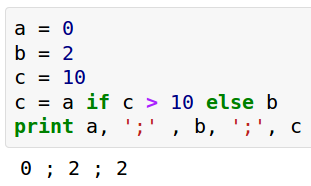
\includegraphics[width=.35\linewidth]{images/04-as-con-var-python.png}
\end{itemize}
\end{frame}

\begin{frame}[fragile]{Asignación en expresiones}
\begin{itemize}
	\item C considera la asignación como un operador más.
	\item Permite incrustar asignación en cualquier expresión.
	\item \textbf{C} Permitido.
 	\begin{lstlisting}[language=C, basicstyle=\scriptsize, escapeinside={|}{|}] 
while ( (c = getchar()) != EOF) {}
	\end{lstlisting}
	\item \textbf{Python:} Sintaxis no lo permite.
	\begin{lstlisting}[language=Python, basicstyle=\scriptsize]
if (d = 5 + c) > 6:
	\end{lstlisting}
	\textbf{Error: Invalid syntax.}
	\item \textcolor{green}{Pro:} Programación más compacta.
	\item \textcolor{red}{Contra:} Fuente de error en la programación. Es fácil equivocarse confundiendo \textbf{==} e \textbf{=}.
\end{itemize}
\end{frame}

%\begin{frame}[fragile]{Precedencia y Asociatividad de Operadores}
%\textbf{Links de interés:}
%\begin{itemize}
%	\item \textbf{C/C++}:\\
%	\url{http://en.cppreference.com/w/cpp/language/operator_precedence}
%	\item \textbf{Python}:\\
%	\url{http://books.google.cl/books?id=qHL5ah1GLoUC\&pg=PA93}
%\end{itemize}
%\end{frame}

\part{Estructuras de Control}
\section{Estructuras de Control}

\subsection{Expresiones Relacionales y Lógicas}
\begin{frame}[fragile]{Expresiones Relacionales y Lógicas}
\begin{itemize}
	\item \textbf{Expresión Relacional:} 
	\begin{itemize}
		\item Usan operador relacional (binario) para comparar los valores de dos operandos. 
		\item Cada operando puede ser una \textbf{expresión aritmética}.
		\item El \textbf{valor resultante} de la expresión es \textbf{booleano}.
		\item Incluye: $==$, $!=$, $<$, $<=$, $>$, $>=$
	\end{itemize}
	\item \textbf{Expresión Booleana:}  
	\begin{itemize}
		\item Consiste en variables, constantes y operadores booleanos.
		\item Se puede combinar con expresiones relacionales.
		\item Incluye: \emph{AND}, \emph{OR}, \emph{NOT} y, a veces, \emph{XOR}.
	\end{itemize}
	\item \textbf{El único valor falso en C es el 0 (cero).}
\end{itemize}
\end{frame}

\begin{frame}{Expresiones Relacionales y Lógicas}
\small
\begin{tabular}{|l|l|l|}\hline \hline
	\multicolumn{3}{|c|}{\textbf{Operadores Relacionales}} \\ \hline
	\textbf{Operador} &\textbf{C} & \textbf{Python}   \\ \hline 
	Igual         & $==$  & $==$  \\  \hline
	Distinto       & $!=$ & $!=$ $<>$ \\  \hline
	Mayor          & $>$ & $>$  \\  \hline
	Menor       & $<$ & $<$ \\  \hline
	Mayor o igual   & $>=$ & $>=$  \\  \hline
	Menor o igual   & $<=$ & $<=$  \\  \hline
	\multicolumn{3}{|c|}{\textbf{Operadores Booleanos}} \\ \hline
	\textbf{Operador} &\textbf{C}  & \textbf{Python}   \\ \hline 
	NOT   & !  &   \textbf{not} \\  \hline
	AND   & $\&\&$  & \textbf{and}  \\  \hline
	OR   & $||$  & \textbf{or}  \\  \hline
\end{tabular}
\end{frame}

\subsection{Estructuras Condicionales}
\frame[containsverbatim]
{
\frametitle{Estructuras de control}
 \begin{itemize}
\item C/Python la ejecución es típicamente secuencial. 
\item Dos tipos básicos de estructuras control:
 \begin{itemize}
\item \textbf{Condicional:} múltiples alternativas de ejecución, controladas por una condición.
\item \textbf{Iterativa:} Ejecución repetitiva de un grupo de sentencias, también controladas por una condición.
  \end{itemize}
\item Se requiere mecanismo de agrupación de sentencias sobre las cuales se ejerce el control: \textbf{composición de sentencias}.
\item En \textbf{C} se usa \emph{\{ \}} 
\item \textbf{Python} compone por indentación.
\end{itemize}
}

\begin{frame}[fragile]{Estructuras de control - Sentencias de selección}
\textbf{if - else if - else}
\begin{columns}[t]
	\begin{column}{5cm}
	\begin{exampleblock}{C}
	\begin{lstlisting}[language=C, basicstyle=\scriptsize, escapeinside={|}{|}] 
if(condición_1) {
    //....
} else if(condición_k) {
    //....
} else {
    //....
}
		\end{lstlisting}\end{exampleblock}
	\end{column}
	\begin{column}{5cm}
		\begin{block}{Python}
		\begin{lstlisting}[language=Python, basicstyle=\scriptsize]
if condición_1:
    #....
elif condición_k:
    #....
else:
    #....
		\end{lstlisting}\end{block}
	\end{column}
\end{columns}
\end{frame}

\begin{frame}[fragile]{Estructuras de control - Sentencias de selección}
\textbf{switch}\\
\begin{exampleblock}{C}
\begin{lstlisting}[language=C, basicstyle=\scriptsize, escapeinside={|}{|}] 
switch(x){ //Debe ser una variable
case x1:                                     
	//.... 
	break; 
case x2: 
	//.... 
	break; 
//.... 
case xN: 
	//.... 
	break;  
default: //opcional
	//....
} 
\end{lstlisting}\end{exampleblock}
\bigskip
\textbf{No existe en Python.}
\end{frame}

\part{Estructuras de Control II}
\section{Estructuras de Control}
\subsection{Estructuras Cíclicas}
\begin{frame}[fragile]{Estructuras de control - Sentencias de iteración}
\textbf{Ciclos controlados por condicion:} \emph{while, do-while}\\
\small
\begin{columns}[t]
	\begin{column}{5cm}
	\begin{exampleblock}{C}
	\begin{lstlisting}[language=C, basicstyle=\scriptsize, escapeinside={|}{|}] 
while(condición) { 
    //...
}

do {
    //...
} while(condición);
		\end{lstlisting}\end{exampleblock}
	\end{column}
	\begin{column}{5cm}
	\begin{block}{Python:}
		\begin{lstlisting}[language=Python, basicstyle=\scriptsize]
while condición: 
    #...
		\end{lstlisting}\end{block}
	\end{column}
\end{columns}
\end{frame}

\begin{frame}[fragile]{Estructuras de control - Sentencias de iteración}
\textbf{Ciclos controlados por contador:} \emph{for}\\
\footnotesize
\begin{exampleblock}{C}
\begin{lstlisting}[language=C, basicstyle=\scriptsize, escapeinside={|}{|}] 
//En general:
for(sentencia_inicial;condición;sentencia_fin_ciclo) { 
    //...
} 
\end{lstlisting}\end{exampleblock}
\begin{columns}[t]
	\begin{column}{5cm}
\begin{exampleblock}{C}
\begin{lstlisting}[language=C, basicstyle=\tiny, escapeinside={|}{|}] 
//Uso corriente
for(i=0; i<N; i++) { 
    //...
} 

//Equivalente a:
i=0;
while(i<N) {
    //...
    i++;
}
		\end{lstlisting}\end{exampleblock}
	\end{column}
	\begin{column}{5cm}
		\begin{block}{Python:}
		\begin{lstlisting}[language=Python, basicstyle=\tiny]
//En general:
for var_iteracion in secuencia:
    #instrucciones ... 
		\end{lstlisting}\end{block}
		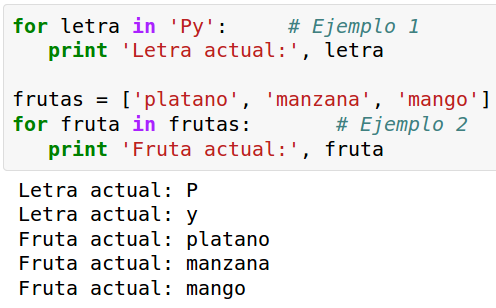
\includegraphics[width=0.65\linewidth]{images/for-python.png}
	\end{column}
\end{columns}
\end{frame}

\subsection{Casos Importantes}
\begin{frame}[fragile]{Corto Circuito o Término anticipado de evaluación}
\begin{itemize}
	\item \textbf{Corto circuito:} Evaluación de una expresión termina antes.
	\item \textbf{C} definen corto circuito para  $\&\&$ y $||$.
	\item Lenguajes como \textbf{Perl y Ruby} evalúan todos sus operandos en una expresión lógica.
	\begin{lstlisting}[language=C, basicstyle=\scriptsize] 
//Si primera condición se cumple, la expresion es true
if((a >= 0) || (b < 10))

//Si primera condición no se cumple, la expresion es false
while ( (c = getchar()) != EOF && c != '\n' )
	\end{lstlisting}
	\item Puede generar inconvenientes en expresiones con efectos colaterales.  
\end{itemize} 
\end{frame}


\begin{frame}[fragile]{Saltos incondicionales}
\begin{itemize}
	\item \textbf{C/Python:}
	\begin{itemize}
		\item \textbf{break:} Permite salir del ciclo más cercano.
		\item \textbf{continue:} Permite pasar al ciclo siguiente.
		\item Se recomienda usarlos con precaución y critero.  
	\end{itemize}
\end{itemize}
\end{frame}

\begin{frame}[fragile]{Saltos incondicionales - Ejemplo}
\footnotesize
\begin{lstlisting}[language=C, basicstyle=\scriptsize, escapeinside={|}{|}] 
int main() {
  int n;
  do {
    printf("Ingrese numero: ");
    scanf("|\%|d", |\&|n);
    if (n < 0)
      break;
    if (n >10) {
      printf("Saltarse el valor.\n");
      continue;
    }
    printf("El numero es: |\%|d\n",  n);
  } while (n != 0);

  return 0;
}
\end{lstlisting}
\end{frame}

%\begin{frame}[fragile]{Manejo de errores y excepciones - try catch}
%\small
%\begin{itemize}
%	\item Transferir el control a lugar donde se maneje un error o excepción, posiblemente interrumpiendo el flujo normal del control.
%	\item \textbf{Ejemplo C/C++:}
%	\begin{lstlisting}[language=C++]
%try {
%    ...  //bloque controlado
%} catch(Overflow) {
%    ...  //Manejar Overflow
%} catch (MathError) {
%    ...  //Manejar MathError
%}
%	\end{lstlisting}
%	
%	\item En \textbf{Python} existe  \textbf{try except}:
%	\begin{lstlisting}[language=Python]
%try:
%    ...  #bloque controlado
%except RuntimeError:
%    ...  #Manejar RuntimeError
%	\end{lstlisting}
%	
%\end{itemize}
%\end{frame}

%\subsection{Subprogramas}
%\begin{frame}[fragile]{Subprogramas}
%\begin{itemize}
%	\item Encapsula código (transparente al invocador).
%	\item Permite reutilizar código.
%	\item Normalmente requiere memoria dinámica de stack.
%	\item Sabores:
%	\begin{itemize}
%		\item Procedimientos o subrutinas (no definen valor de retorno).
%		\item Funciones (con retorno).
%		\item Métodos y constructores en OO. 
%	\end{itemize}
%\end{itemize}
%\end{frame}
%
%\begin{frame}[fragile]{Subprogramas en C/C++ - Funciones}
%\begin{itemize}
%	\item Se puede separar interfaz (prototipo) de implementación.
%	\item \textbf{Interfaz (prototipo):} Sólo define existencia y formato de función. Suficiente para ser invocada.
%	\begin{lstlisting}[language=C++]
%tipo_retorno funcion(parametros con o sin nombre);
%//Ejemplo:
%float potencia(float, float);
%//....
%
%calculo = x * potencia(y, 2.5);
%	\end{lstlisting}
%	\item \textbf{Implementación:} Define implementación de código de función.
%	\begin{lstlisting}[language=C++]
%tipo_retorno funcion(parametros con nombre) {
%	//Implementacion...
%}
%//Ejemplo:
%float potencia(float base, float exp) {
%	//Implementacion...
%}
%	\end{lstlisting}
%\end{itemize}
%\end{frame}
%
%\begin{frame}[fragile]{Subprogramas en Python - Funciones}
%\begin{itemize}
%	\item \textbf{Python} sólo permite implementación, no prototipos.
%	\begin{lstlisting}[language=Python]
%def nombre_funcion(parametros):
%    #...Implementacion
%    return [expresion]
%
%#Ejemplo:
%	\end{lstlisting}
%	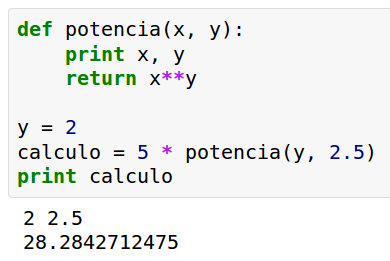
\includegraphics[width=.7\linewidth]{images/funcion-python.png}
%\end{itemize}
%\end{frame}

\end{document}
